\documentclass{article}

\usepackage{fontspec}
\setmainfont{Libertinus Serif}
\usepackage[margin=1in]{geometry}

\usepackage{tikz}
\usetikzlibrary{arrows.meta}
\usetikzlibrary{positioning}
\usetikzlibrary{quotes}

\newcommand{\person}[5]{%
    \begin{tabular}{c}
        #1\\
        \textsc{#2} \\[1ex]
        \emph{#3} \\[1ex]
        #4 \\
        {\small #5}
    \end{tabular}%
}

\def\Santiago{\person
{Fray Francisco de}
{Santiago}
{Voces, las de la capilla} 
{Pre-1644 Christmas, Seville Cathedral (or Lisbon)}
{Text incipits in 1649 catalog of João IV}
}

\def\Padilla{\person
{Juan}
{Gutiérrez de Padilla}
{Voces, las de la capilla}
{1657 Christmas, Puebla Cathedral}
{Music in partbooks, Puebla Cathedral Archive}
}

\def\Jalon{\person
{Luis Bernardo}
{Jalón}
{Cantores de la capilla}
{1647 Epiphany, Seville Cathedral}
{Text in poetry imprint, sole exemplar, Puebla private collection}
}

\newcommand{\relation}[1]{\parbox{8em}{\raggedright\small\itshape#1}}
\def\SantiagoToPadilla{\relation{Santiago MC Seville while Padilla MC Cádiz,
1616--22}}
\def\SantiagoToJalon{\relation{Jalón assists then succeeds Santiago as Seville MC after
death, 1644}}
\def\JalonToPadilla{\relation{Jalón text known in Puebla through imprint}}

\begin{document}
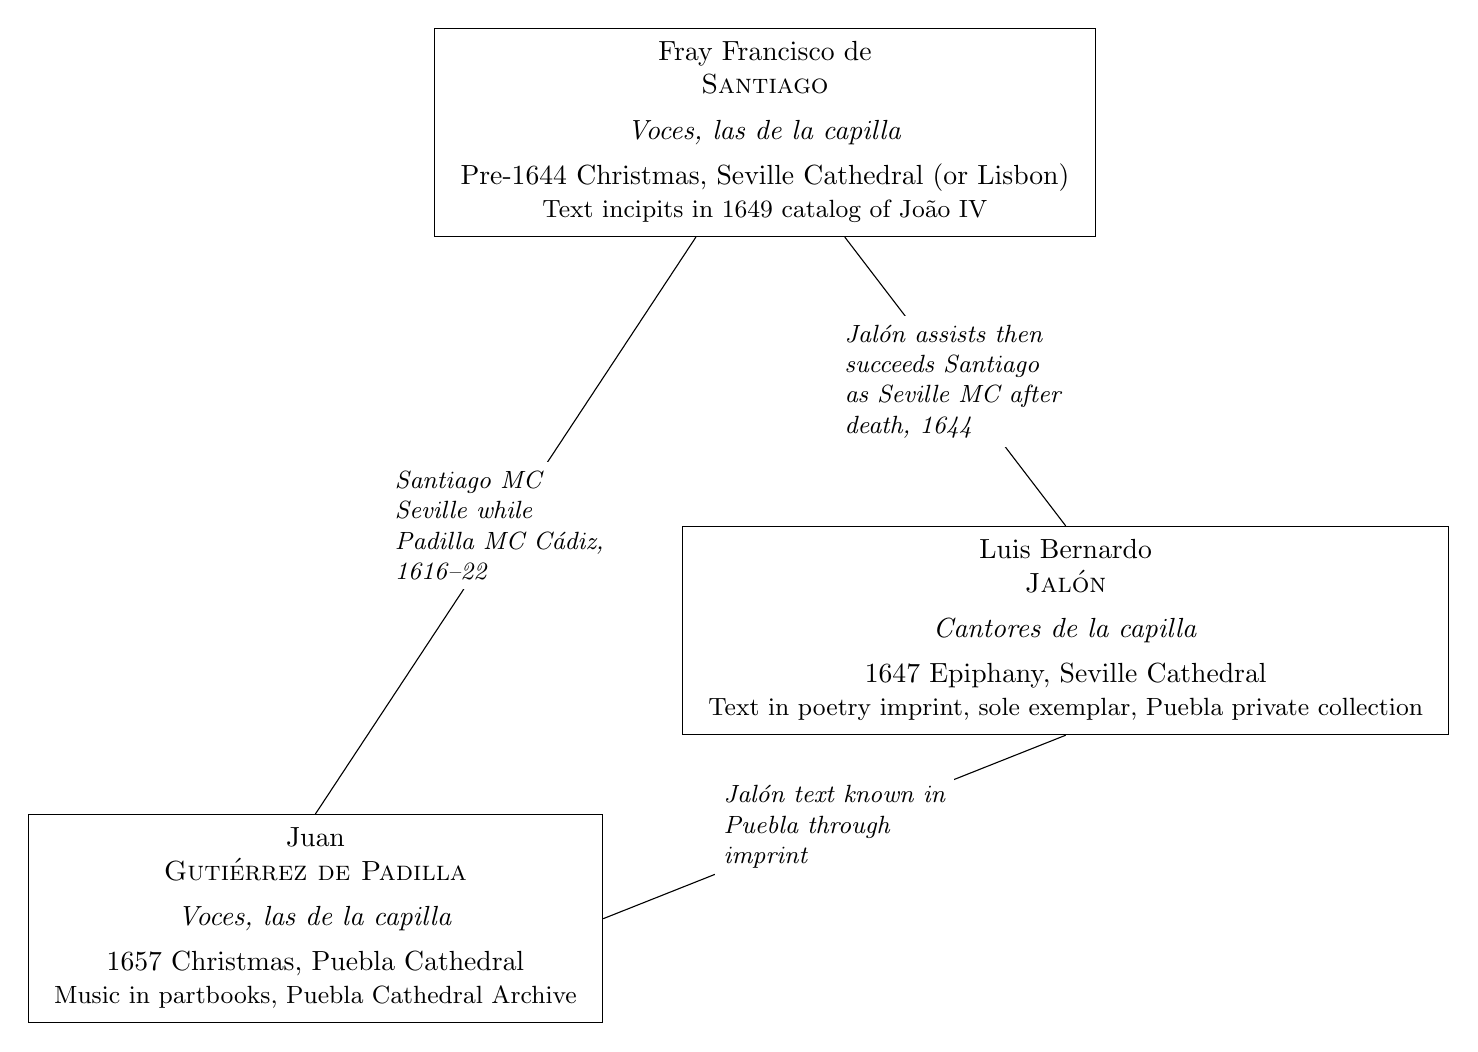
\begin{tikzpicture}[level distance=18em, 
                    sibling distance=6em,
                    every node/.style={draw},
                    edge from parent/.style={draw=none},
                    every edge quotes/.style={draw=none,fill=white}]

    \node (s) {\Santiago}
        child { node[right] (j) {\Jalon} }
        child { node[left, below left=of j] (p) {\Padilla} };
    \draw[-] (s)        edge ["\SantiagoToPadilla"  midway] (p.north);
    \draw[-] (s)        edge ["\SantiagoToJalon"    midway] (j.north);
    \draw[-] (j.south)  edge ["\JalonToPadilla"     midway] (p.east);
\end{tikzpicture}
\end{document}

